\subsection{Случайная величина.}
\deff{Случайная величина} или численная характеристика каждого элементарного исхода --- это отображение, $\xi: \Omega \rightarrow \mathbb{R}$, которое сопоставляет каждому элементарному исходу какое-то число.\\
\textbf{Пример:}

\begin{enumerate}
    \item $D = \{1,2,\ldots,6\}$. Возьмем $\Omega = D^2$. Например, человек бросает два игральных кубика. Тогда, очевидно, $p(\langle i,j\rangle) = \cfrac{1}{36}$. И тогда он задает функцию случайной величины, например, как $\xi(\langle i,j \rangle) = i+j$.

    \item Возьмем случайный граф $G$ на $n$ вершинах. $\xi(G) = $ количеству компонент связности. Или  $\xi(G) = $ количеству ребер в этом графе.

    \item Давайте кидать игральный кубик и сопоставим каждой выпадающей гране число равное количеству точек на этой грани.\\То есть $\Omega = \{1,2,\ldots,6\}$, $\xi (i) = i$. 
    \item  $\Omega =\{1,2,\ldots,6\}; E = \{2,4,6\}$. $x_E(w) = \begin{cases}
        1, w\in E\\
        0, w\notin E 
    \end{cases}$
\end{enumerate}

Возьмем какие-то $\Omega, p, \xi$:

$\left[\xi = i\right] = \{w|\xi(w)=i\}\subset \Omega$ --- \deff{множество элементарных исходов}, случайная величина, которых равна i. 

\deff{def:} $f_{\xi}:\mathbb{R}\rightarrow \mathbb{R}$ --- \deff{дискретная плотность вероятности $\xi$}.
$$P([\xi=i])=P(\xi=i) = f_{\xi}(i) =\sum\limits_{w \in [\xi=i]}p(w)$$
\textbf{Дискретная плотность вероятности} --- это функция, которая говорит нам, насколько вероятно каждое из этих отдельных значений, которые может принимать случайная величина. Другими словами, она присваивает вероятность каждому возможному исходу.

Немного поменяем и получим $\left[\xi \leq i\right] = \{w|\xi(w)\leq i\}\subset \Omega$.
$$P([\xi \leq i])=P(\xi\leq i) = F_{\xi}(i)$$
\deff{def:} $F_{\xi}:\mathbb{R}\rightarrow \mathbb{R}$ --- \deff{функция распределения}. У дискретной случайной величины функция распределения ступенчатая. Например:

\begin{center}
    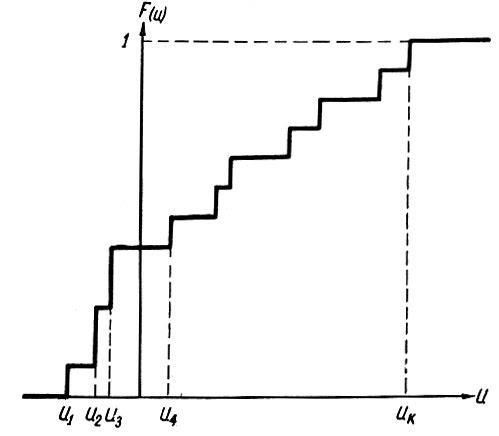
\includegraphics[width = 10cm]{assets/2_1_1.jpg}
\end{center}

\subsection{Мат. ожидание.}
\deff{Математическое ожидание} --- среднее значение случайной величины. 

$E_{\xi} =\sum\limits_{w}p(w) \xi(w)=\sum\limits_{i}i\cdot P(\xi=i)$.

Дальше А.С. использует 3 вида обозначений:

1. $E_{\xi}$ 2. $E(\xi)$  3. $E \xi$ --- не боимся, это одно и то же.



\thmm{Теорема (линейность мат ожидания)}
$$E \lambda\xi = \lambda E_{\xi}\quad E_{(\xi + \eta)} = E_{\xi} + E_{\eta}$$


\textbf{Доказательство:}
$$E\lambda\xi = \sum\limits_{w}p(w) \cdot \lambda \xi(w) = \lambda \sum\limits_{w}p(w)  \xi(w)=\lambda E_{\xi}$$
$$E(\xi+\eta) = \sum\limits_{w}p(w) (\xi(w) + \eta(w))  = \sum\limits_{w}p(w) \xi(w) +\sum\limits_{w} p(w)\eta(w) = E(\xi) +E(\eta) $$
\hfill Q.E.D.

\textbf{\uline{МАТ. ОЖИДАНИЕ ВСЕГДА ЛИНЕЙНО!!!}}

\subsection{Незав. случайные величины} 

$\xi,\eta$ - \deff{независимы}, если $[\xi = a], [\eta = b]$ --- независимы $\forall a,b$.

Эквивалентное утверждение --- $[\xi\leq a], [\eta\leq b]$ --- независимы $\forall a,b$.

Иначе говоря, две случайные величины называются \emph{независимыми}, если по значению одной нельзя сделать выводы о значении другой.

\thmm{Теорема (о мультипликативности мат. ожидания)}

$\xi,\eta$ --- независимы $\Rightarrow E(\xi\cdot\eta)=E_{\xi}\cdot E_{\eta}$.

\textbf{Доказательство:}

$$E_{(\xi\cdot \eta)}=\sum\limits_{a}a P(\xi,\eta = a) = 
\sum\limits_{a}a\sum\limits_{\forall i,j: \,i\cdot j= a \, i \in R_{\xi},j\in R_{\eta}}P(\xi = i, \eta = j) =$$ $$= \sum\limits_{a}\sum\limits_{i}\sum\limits_{j} aP(\xi=i) P(\eta = j) = \sum\limits_{i}iP(\xi=i)\cdot \sum\limits_{j}jP(\eta=j) = E_{\eta}\cdot E_{\xi}$$
\hfill Q.E.D.

\subsection{Дисперсия случайной величины.}
$D_{\xi} = Var(\xi)$ --- \deff{дисперсия} случайной величины. 
$$D_{\xi}= E((\xi - E_{\xi})^2)= E_{\xi^2}-(E_{\xi})^2$$
\textbf{Дисперсия случайной величины} --- это мера того, насколько сильно разбросаны значения этой случайной величины вокруг её математического ожидания (среднего значения). Другими словами, она показывает, насколько "широко" распределение вероятностей случайной величины.

\thmm{Теорема (свойства дисперсии).}
Если $\xi,\eta$ - независимы:
$$D_{c\eta} = c^2 D_{\eta}\quad D_{\xi+\eta}=D_{\xi}+D_{\eta}$$

\textbf{Доказательство тривиально из линейности мат. ожидания}